% Copyright (C) 2014-2016 by Thomas Auzinger <thomas@auzinger.name>

\documentclass[draft,final]{vutinfth} % Remove option 'final' to obtain debug information.

% Load packages to allow in- and output of non-ASCII characters.
\usepackage{lmodern}        % Use an extension of the original Computer Modern font to minimize the use of bitmapped letters.
\usepackage[T1]{fontenc}    % Determines font encoding of the output. Font packages have to be included before this line.
\usepackage[utf8]{inputenc} % Determines encoding of the input. All input files have to use UTF8 encoding.

% Extended LaTeX functionality is enables by including packages with \usepackage{...}.
\usepackage{amsmath}    % Extended typesetting of mathematical expression.
\usepackage{amssymb}    % Provides a multitude of mathematical symbols.
\usepackage{mathtools}  % Further extensions of mathematical typesetting.
\usepackage{microtype}  % Small-scale typographic enhancements.
\usepackage[inline]{enumitem} % User control over the layout of lists (itemize, enumerate, description).
\usepackage{multirow}   % Allows table elements to span several rows.
\usepackage{booktabs}   % Improves the typesettings of tables.
\usepackage{subcaption} % Allows the use of subfigures and enables their referencing.
\usepackage[ruled,linesnumbered,algochapter]{algorithm2e} % Enables the writing of pseudo code.
\usepackage[usenames,dvipsnames,table]{xcolor} % Allows the definition and use of colors. This package has to be included before tikz.
\usepackage{nag}       % Issues warnings when best practices in writing LaTeX documents are violated.
\usepackage{todonotes} % Provides tooltip-like todo notes.
\usepackage{hyperref}  % Enables cross linking in the electronic document version. This package has to be included second to last.
\usepackage[acronym,toc]{glossaries} % Enables the generation of glossaries and lists fo acronyms. This package has to be included last.


\newenvironment{conditions}
{\par\vspace{\abovedisplayskip}\noindent\begin{tabular}{>{$}l<{$} @{${}={}$} l}}
	{\end{tabular}\par\vspace{\belowdisplayskip}}

% Define convenience functions to use the author name and the thesis title in the PDF document properties.
\newcommand{\authorname}{Rebeka Koszticsak} % The author name without titles.
\newcommand{\thesistitle}{Illustrative Thumbnails} % The title of the thesis. The English version should be used, if it exists.

% Set PDF document properties
\hypersetup{
	pdfpagelayout   = TwoPageRight,           % How the document is shown in PDF viewers (optional).
	linkbordercolor = {Melon},                % The color of the borders of boxes around crosslinks (optional).
	pdfauthor       = {\authorname},          % The author's name in the document properties (optional).
	pdftitle        = {\thesistitle},         % The document's title in the document properties (optional).
	pdfsubject      = {Subject},              % The document's subject in the document properties (optional).
	pdfkeywords     = {a, list, of, keywords} % The document's keywords in the document properties (optional).
}

\setpnumwidth{2.5em}        % Avoid overfull hboxes in the table of contents (see memoir manual).
\setsecnumdepth{subsection} % Enumerate subsections.

\nonzeroparskip             % Create space between paragraphs (optional).
\setlength{\parindent}{0pt} % Remove paragraph identation (optional).

\makeindex      % Use an optional index.
\makeglossaries % Use an optional glossary.
%\glstocfalse   % Remove the glossaries from the table of contents.

% Set persons with 4 arguments:
%  {title before name}{name}{title after name}{gender}
%  where both titles are optional (i.e. can be given as empty brackets {}).
\setauthor{}{\authorname}{}{female}
\setadvisor{Dr. techn.}{Manuela Waldner}{Msc.}{female}

% For bachelor and master theses:
%\setfirstassistant{Pretitle}{Forename Surname}{Posttitle}{male}
%\setsecondassistant{Pretitle}{Forename Surname}{Posttitle}{male}
%\setthirdassistant{Pretitle}{Forename Surname}{Posttitle}{male}

% For dissertations:
\setfirstreviewer{Pretitle}{Forename Surname}{Posttitle}{male}
\setsecondreviewer{Pretitle}{Forename Surname}{Posttitle}{male}

% For dissertations at the PhD School and optionally for dissertations:
\setsecondadvisor{Pretitle}{Forename Surname}{Posttitle}{male} % Comment to remove.

% Required data.
\setaddress{Address}
\setregnumber{1325492}
\setdate{01}{01}{2001} % Set date with 3 arguments: {day}{month}{year}.
\settitle{\thesistitle}{Illustrative Thumbnails} % Sets English and German version of the title (both can be English or German).
%\setsubtitle{Optional Subtitle of the Thesis}{Optionaler Untertitel der Arbeit} % Sets English and German version of the subtitle (both can be English or German).

% Select the thesis type: bachelor / master / doctor / phd-school.
% Bachelor:
\setthesis{bachelor}
%
% Master:
%\setthesis{master}
%\setmasterdegree{dipl.} % dipl. / rer.nat. / rer.soc.oec. / master
%
% Doctor:
%\setthesis{doctor}
%\setdoctordegree{rer.soc.oec.}% rer.nat. / techn. / rer.soc.oec.
%
% Doctor at the PhD School
%\setthesis{phd-school} % Deactivate non-English title pages (see below)

% For bachelor and master:
\setcurriculum{Media Informatics and Visual Computing}{Medieninformatik und Visual Computing} % Sets the English and German name of the curriculum.

% For dissertations at the PhD School:
\setfirstreviewerdata{Affiliation, Country}
\setsecondreviewerdata{Affiliation, Country}


\begin{document}
	
	\frontmatter % Switches to roman numbering.
	% The structure of the thesis has to conform to
	%  http://www.informatik.tuwien.ac.at/dekanat
	
	\addtitlepage{naustrian} % German title page (not for dissertations at the PhD School).
	\addtitlepage{english} % English title page.
	\addstatementpage
	
	\begin{danksagung*}
		\todo{Ihr Text hier.}
	\end{danksagung*}
	
	\begin{acknowledgements*}
		\todo{Enter your text here.}
	\end{acknowledgements*}
	
	\begin{kurzfassung}
		\todo{Ihr Text hier.}
	\end{kurzfassung}
	
	\begin{abstract}
		Thumbnails are used to display a list of open windows or tabs when switching between them on the computer
		and on mobile devices. 
		These images make it easier to recognize the opened applications, and help to find the needed window quicker. Thumbnails display however only a screenshot
		of the windows, so they get potentially confusing if there are more opened windows or if the
		same application is opened multiple times. Depending on the resolution of the display, the
		screenshot size decreases as the number of opened windows increases. Furthermore,
		within the same application (like MS Office World) the screenshots are similar in appearance
		(eg.: white paper and tool bar), but the important text is not readable.
		There are several approaches that filter the important areas of the images to make editting
		less obvious or enhance the main region. In this bachelor thesis an application
		is implemented that uses these methods on the screencaptured
		images. The less important
		areas of the screenshots are cut off, and only if no more irrelevant information remains, a conventional downsampling algorithm is applied.
		So the thumbnails show only salient information,
		which makes them more illustrative and easier to fulfill their purpose.
	\end{abstract}
	
	% Select the language of the thesis, e.g., english or naustrian.
	\selectlanguage{english}
	
	% Add a table of contents (toc).
	\tableofcontents % Starred version, i.e., \tableofcontents*, removes the self-entry.
	
	% Switch to arabic numbering and start the enumeration of chapters in the table of content.
	\mainmatter
	
	\chapter{Introduction}
	With the increased use of mobile devices and reliance on multi-tasking thumbnails are becoming increasingly important.
	Thumbnails appear when switching between tasks, representing the concurrent windows i.e. the running applications.
	To keep a continuous and effective workflow, it is essential to make the process of switching as fast and smooth as possible by allowing the user to quickly identify and choose between the given tabs. 
	However, the current thumbnail system is not fit for this purpose. 
	Due to the fact that standard thumbnail applications simply take the screenshot of each application and present them in a smaller size, the relevant parts of the window are no longer recognizable. 
	For example, the user interface widgets, especially in case of the multiple windows of the same application, take up valuable place that could otherwise be used to present more important content elements, such as actual file names or other unique characteristics of the window.
	Furthermore with the use of tablets, smart phones and smart watches the display, thus the thumbnail size needs to shrink even more, but the original calculation algorithm does not take this into account.
	Figure~\ref{fig:introo} shows a possible output of the current (Figure~\ref{fig:introo:org}) and the new (Figure~\ref{fig:introo:res}) thumbnail creating algorithms.\par 
	\begin{figure}[h]
		\centering
		\begin{subfigure}[b]{0.45\columnwidth}
			\centering
			
\includegraphics[width=\textwidth]{orgBlizzard}
			\subcaption{Currently used thumbnail}
			\label{fig:introo:org}
		\end{subfigure}
		\begin{subfigure}[b]{0.45\columnwidth}
			\centering
			
\includegraphics[width=\textwidth]{resultBlizzard}
			\subcaption{Thumbnail created by the new algorithm}
			\label{fig:introo:res}
		\end{subfigure}
		\caption{The result using the two different approaches}
		\label{fig:introo} % \label has to be placed AFTER \caption (or \subcaption) to produce correct cross-references.
	\end{figure}
	This project introduces a new approach using seam carving to make thumbnails more illustrative even on small displays.
	Seam carving is a special re-sampling method, where not necessarily straight lines are determined, and the least important of them are then eliminated.
	The definition of importance depends on the implementation, but it in any case evaluates color changes and identifies the edges that shape the outline of the element on the source image.
	Following a similar logic, the algorithm presented in this thesis uses a customized seam carving method.
	Furthermore, it takes into account that the given input is essentially a screenshot thus will probably contain some UI elements on the picture.
	Additionally, considering that letters are more common on computer screens than on usual images, the text content is also investigated to calculate its salient regions.
	
	\section{Definition of the word illustrative} 
	To provide satisfactory results a detailed and clear definition of the word illustrative is needed.
	Not only it influences the calculation of the pixel and region saliency value, but also acts at the selection of result outputs, and is useful for future software development.
	Also, for a fitting definition it needs to be taken into account that in this case the seam carving algorithm is used for screenshots and not for usual photographs.\par 
	The expression 'illustrative thumbnail' also comprehends that it is able to represent more information on a same sized picture than the other not illustrative thumbnail.
	Unlike usual visual features observed on real world images, such as color changes and location of edges, as mentioned above, computer screens have additional special properties that require further consideration.
	For example, most screenshots include UI widgets, that are classified as not illustrative.
	Namely, it is rarely the case that the relevant part of an application is its UI and not its the actual content processing features, additionally, the identification of the a window in question is also possible by reading its title.
	Furthermore text data has on the computer screen more important role then usual pictures.
	To transmit as much information as possible, text data is not allowed to get damaged, i.e. even after size reduction it needs to stay readable.\par 
	Summing up, in this project a thumbnail is called 'illustrative' if its informative content preserves.
	To measure this property, contrast values, color changes, location of edges, text data and the presence of UI elements are evaluated and considered.            
	
	\chapter{Related Work}
	There are several image processing algorithms that can be helpful at creating illustrative thumbnails.
	The main difference between thus algorithms is whether they consider the input as an actual application window or just as a regular image.
	Therefore, this section is divided into two parts.
	The first one discusses algorithms with UI processing segments.
	Algorithms, invented for resampling natural images, are examined in the second section. 
	Moreover, there are two classes of information presentation methods are to be distinguished, namely, simple resizing and collages, the latter combining the most important parts of the image. 
	In the following, these methods are compared.
	
	\section{Processing as UI}
	When the input is a screenshot, there is a high chance that the usual UI elements, like buttons and menu bars, are shown on the screen.
	Exceptions for this are only cases when graphics, images, videos or application are presented, such as video games, gallery program or video players.
	Such applications tend to hide all UI elements and operate in 'fullscreen' mode, or use a redefined UI e.g. game menu bars.\par
	Labeling the image parts as content and non-content, the metadata about the UI elements can be helpful.
	Chang et al. ~\cite{chang2011associating} uses already existing accessibility APIs, tested on Mac OS X and on Microsoft Windows, to segment UI and non-UI data. 
	Matching the metadata with the screen content provides a fast and robust result about the location of any kind of UI content.
	There are however several disadvantages, that need to be taken into account when using such APIs.
	The range and the granularity of the support is often not wide enough.
	The use of an accessibility API is unable to ensure that every UI elements are recognized, because some metadata are not reachable or they will be ignored by the application.\par
	Consequently, Prefab ~\cite{dixon2010prefab} uses an adapted of such prototypes. 
	In the database, models and  prototypes of common UI elements are saved.
	The (components of) UI elements are then matched with the prototypes from the database, allowing a consequent access to the predefined metadata.
	Since the Prefab system is able to split complex widgets to their constructing elements, the database does not need to be unnecessary big, though it is still able to cover the most common UI elements.
	In the case of special or rare UI widgets, like in a video game application or elements of a not widely used software, the system fails to recognize them, since these rare widgets are not included in the given database.\par
	Sikuli ~\cite{yeh2009sikuli} offers a solution not only for the incompleteness of such database, but for issues around granularity, too.
	It uses its own templates just like the Prefab system, but only in case of small icons and widgets.
	Since in case of larger objects template matching would be too expensive in terms of time and space, after accomplishing a training pattern, the Sikuli system is able to create new object models too.
	Although in the original application this feature is used for another purpose, i.e. to reduce matching costs, it can effectively used to solve the problem of database and granularity.
	With other words, Sikuli allows the expansion of the database and thus creating a more detailed database entries.\par	
	On the other hand, in case of accessibility APIs, it is not only the availability of the metadata that may cause problems, but also it does not provide information about the actual visibility of the UI elements.
	One window or rather one widget can overlap with or even fully cover another, some content can be out of the range of the borders of the screen etc.    
	The algorithm of Dixon et al. ~\cite{dixon2011content} is built on the Prefab system, but additionally it creates a hierarchical tree of the widgets. 
	The content is found at the leafs, and the parents are the widget, where the child is built in.
	With the help of this tree the order of the UI elements gets clear, and so the misleading information can be eliminated.\par
	After the labeling of the UI elements correctly, they can be manipulated as needed.
	They can cut off as whole or processed according to the information content.
	Mirkamali et al. ~\cite{mirkamali2015object} invented an algorithm that eliminates the picture objects and fill their place with the texture of the object behind them using the z-buffer information.
	The tree mentioned above works as a z-buffer in this case.
	With this cut off algorithm, unnecessary widgets can easily be eliminated and more important elements of the UI can thus get more visible.\par
	According to the definition of "illustrative", the UI elements of a screen in any case are to be excluded, consequently the segmentation of the UI elements is not required.
	Although the Prefab and Sikuli systems are proved to be helpful at distinguishing between UI and content parts of the image, these approaches have their disadvantage at their reliance on database usage and at their slow template matching performance. 
	Furthermore they are actually designed for another purpose, namely to segment and classify UI elements, so before their employment significant reworking is needed.
	Since it is not essential to know, which exact widgets appear on the screen, and processing their actual content may cause performance issues, the use of the above methods would overcomplicate the application without providing noteworthy advantages.
	
	\section{Processing as a regular picture}
	There are several information retrieving methods for processing images with any kind of content.
	Furthermore, these methods can also handle a series of important tasks such as interesting point recognition, Region of Interest (ROI) selection, image or feature composition, i.e. tasks that are in order to make any kind of images more illustrative.
	Based on the type of input data, there are two groups of the above algorithms that will be discussed in the following sections.
	The first category works with more than one picture at the same time.
	Its strength is to choose single features that best represents the whole input data. 
	In exchange it is likely that no input image will be recognizable on the result.
	To the contrary, there are the methods in the second group that take only one picture for input and process it as one unit.
	The resulting image is similar to the input data, however thus it is likely that not only the unimportant but also the areas with high information ratio are damaged.
	Finally, in the subsection below some approaches are presented that assist with the work of both of the above mentioned groups.
	
	\subsection{Collage creating methods} 
	A collage is an assembled image, containing parts of a bunch of input images and being representative for the whole input data.
	There are two cases by creating  more illustrative thumbnails where such methods can be helpful.
	On the one hand the actual information of a screenshot image is presented only in few regions of the picture.
	Many parts, for example UI elements, space between the content etc., can be ignored. 
	The other way around the content can be retrieved in form of ROIs, and afterwards they can be combined arbitrary.
	On the other hand thumbnails for desktop switching can be easily generated using collage creator algorithms, where the input is screenshots of the open applications of the desktop instead of some ROIs of one screen.\par
	For a representative collage the most important task is to choose the best images, which information content covers the whole input data.
	Rother et al. ~\cite{rother2006autocollage} takes the parameters representativeness, importance costs, transition cost and object sensitivity into account.
	\[ E(L)=E_{rep}(L)+w_{imp}E_{imp}(L)+w_{trans}E_{trans}(L)+w_{obj}E_{obj}(L) \]
	Representativeness means being interesting in this case.
	A picture tends to have high representativeness value, if there are many special textures on it, and if it is not similar to the rest of the data (so that no image is chosen twice).
	Importance cost evaluates and collects the ROIs of the input.
	While transition cost stands for the smooth transition between every two images.
	At last, the parameter object sensitivity holds the results of object recognition, and it helps in the arrangement, that every object has a reasonable placement.\par
	Egorova et al. ~\cite{egorova2008collage} concentrates however only at the first two parameters above.
	It clusters the images according to their source and the time, and measures the quality.
	Thank for the clustering, by the choice of the final images it is clear,  which images are the same or have similar content.
	This feature, accordingly modified, can be useful by sorting ROIs of a screenshot, i.e.: text content, image content etc. or of the running applications of the desktop, i.e.: textprocessing, gallery application etc.
	The parameter quality summarizes the value of the results of the following calculations: blurriness, compression, contrast and color balance.
	Since in this case only screenshots, thus computer generated pictures, can be the input, these measurements invented for camera data would provide less meaningful results than the algorithm above.\par 
	\begin{figure}[h]
		\centering		
		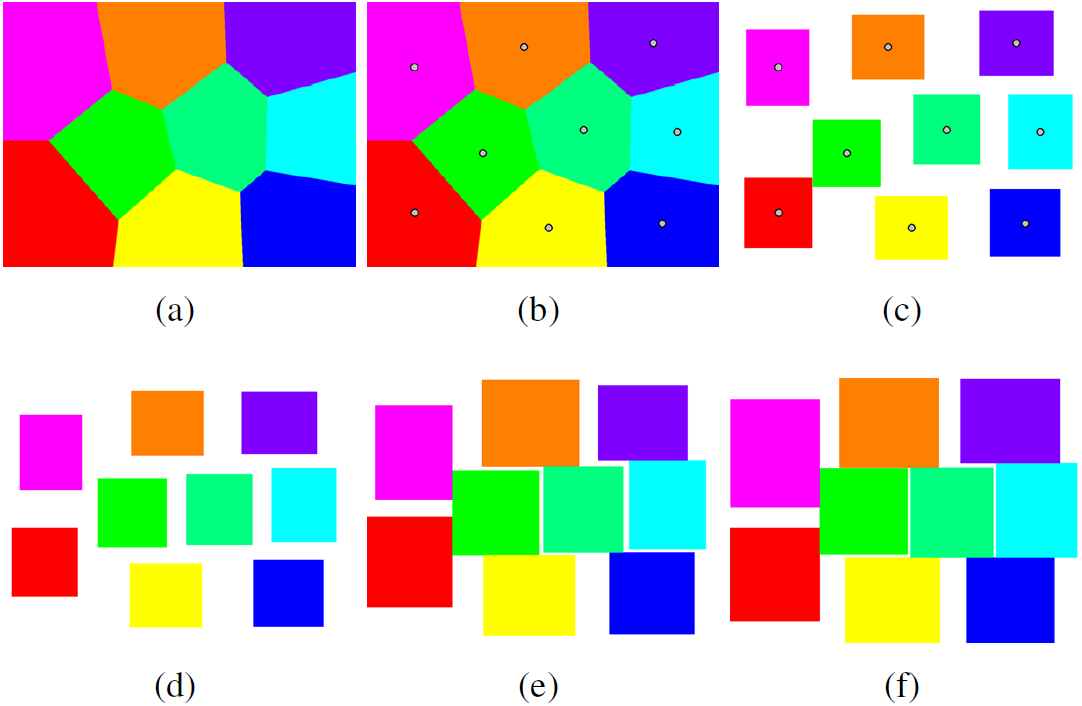
\includegraphics[width=0.5\textwidth]{ROIpacking}
		\caption{The whole ROI packing process ~\cite{lee2010mobile} (a) K-means clustering (b) ROI's center at the beginning of the algoritm (c) Layout of the ROIs at the beginning of the algorithm (d) Shifting of the ROIs (e) Expanding the ROIs (f) Output after some iterations}
		\label{fig:ROIpacking}
	\end{figure}
	Having the best ROIs for the collage the last task is to merge them into one output picture.
	For this purpose Lee et al. ~\cite{lee2010mobile} uses a method called ROI packing.
	First the central point of every ROI is selected and every pixel on the canvas needs to get assigned to one of them using the K-Means algorithm.
	After that the ROIs can be placed on the area calculated for them.
	To fill the place between the ROIs they are increased, keeping the aspect ratio, until they overlap. 
	Then every ROI is shifted to the middle of its area.
	This method is repeated until there are no further increases in the ROI anymore.
	To fill the white areas and eliminate any empty place, neighboring ROIs are allowed to partially cover each other.
	Figure~\ref{fig:ROIpacking} shows the different steps of the ROI packing algorithm.\par 
	Collage methods are excellent at representing a large image dataset in a small place.
	They work with numerous input data, take the most important parts of them and create a new image, that is not similar to any previous one.
	That is why they are more useful for making a thumbnail for a desktop while not being much so in case of applications.
	Even though with taking the most important ROIs of one screen it would be possible to create a  more illustrative image than any other, since the important content could stay large and so well readable, classic collage assembly methods were developed for natural images.
	Screenshot collages have however different requirements for image and text regions.
	In addition, cutting a screen apart and arranging its parts willingly has a potentially confusing result for the user, requiring them to spend even more time with the screen recognition.
	
	\subsection{Resampling methods}
	To attain a constant relative position among regions, applying a resampling method is more effective than the above described collage creating approaches.
	Resampling means that some equally distributed parts of the image will be eliminated, thus, unlike by the collage algorithms, all remaining areas will have the same relation to each other.
	Therefore, the image itself remains recognizable because it has a highly similar appearance, in spite of having the most important areas less readable.\par 
	To select the invariable areas Chen et al. ~\cite{chen2003visual} suggests various attention models that are able to define the so-called Attention Objects (AO).
	AOs are usually real-world objects that due to their familiarity, shape, color etc., attract the human eye.
	AOs can easily be parametrized using three values: ROI, Attention Value (AV) and Minimal Perceptible Size (MPS).
	The attention models fit the AOs into their context.
	The algorithm works with three different attention models at the same time: saliency, face and text attention.
	The most important areas can be detected according to the importance value of each given pixel.\par 
	\begin{figure}[h]
		\centering		
		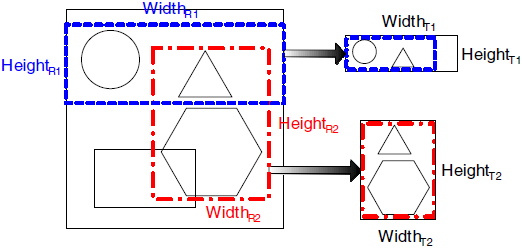
\includegraphics[width=0.5\textwidth]{useOfAOs}
		\caption{Possible solutions of the algorithm of Chen et al. ~\cite{chen2003visual}}
		\label{fig:useOfAOs}
	\end{figure}
	The approach above, after careful calculations, chooses the only area that contains the highest possible amount of AOs.
	To accomplish this, some possibly important AOs have to be ignored and cut off, like shown on Figure~\ref{fig:useOfAOs}.
	With Feature-aware Texturing described in ~\cite{gal2006feature} this does not have to be the case.
	The algorithm expects an input image and a feature mask.
	A grid is generated, which lies on the input image.
	This grid can be modified in an optional shape, but the gridpoints on the feature mask are not allowed to change their proportion to each other.
	In that way the picture elements between the AOs fill the new shape, but the AOs get barely distorted, illustrated on Figure~\ref{fig:fat}.\par 
	 \begin{figure}[h]
		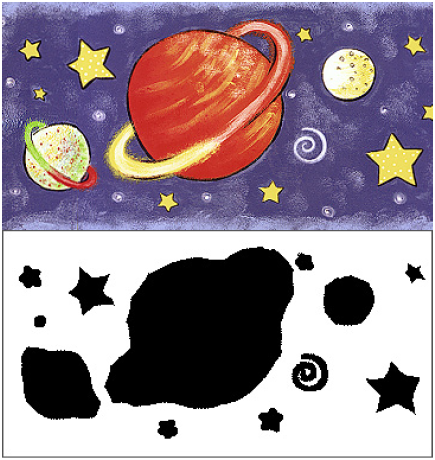
\includegraphics[width=.3\textwidth]{featureAwareTexturing1}\hfill
		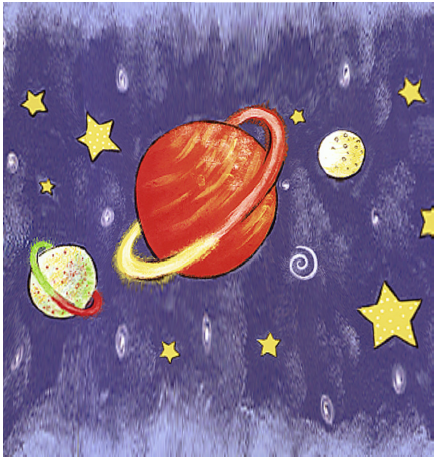
\includegraphics[width=.3\textwidth]{featureAwareTexturing2}\hfill
		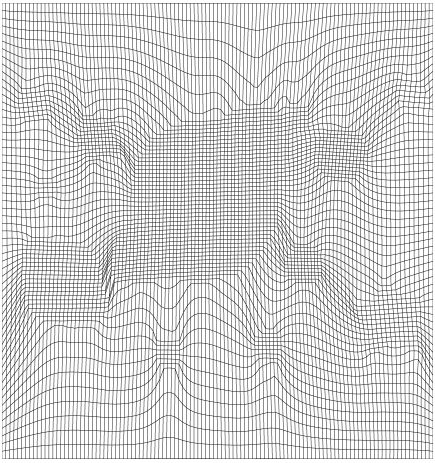
\includegraphics[width=.3\textwidth]{featureAwareTexturing3}
		\caption{The resulting image and grid from a certain input image and its feature mask of the Feature-aware Texturnig algorithm ~\cite{gal2006feature} }
		\label{fig:fat}
	\end{figure}
	A detailed importance is essential at creating thumbnails, since a screen usually contains a greater amount of sensitive information.
	For example, a text can get easily destroyed, since they do not include such a clear focus point as regular pictures, where the density of ROIs is high. 
	But the algorithms described above has aspects like face recognition and grid determination that over-complicate the calculations, causing performance issues without reaching better quality.
	A face on a computer screen is not as frequent as on usual photos, and in addition it is not as sensitive as for example a text data.
	In the case of down sampling a human face can stay recognizable, whereas texts quickly become illegible. 
	With a grid the input image can get reshaped to any other form with no additional damage to the important areas.
	But it is meant to form the input in completely other shape, not for resize it according to aspect ratio.
	Some aspects however, like definition of AOs, could expand the actual used approaches, this possibility will be discussed in the \hyperref[futureWork]{future work} section.
	
	\subsection{Feature combining methods}
	All the above mentioned approaches work with some kind of feature combining algorithms.
	After choosing the relevant areas that need to stay recognizable also on the resulting image, they are merged into one output picture according to their methods.
	It is usual in this process  that some artifacts show up near the joining area.\par 
	A possible solution for this problem is the Poisson equation for image processing, introduced by Perez et al. ~\cite{perez2003poisson}.
	A modified Poisson equation using a guidance field needs to be solved for every color in the color space where the guidance field is calculated from the gradients of the input image.
	This algorithm is actually invented for seamless cloning, but it is helpful when some not-neighboring parts of the same image need to be placed near each other.
	To make the Poisson calculation more efficient an algorithm suggested by Hussain et al. ~\cite{hussain2016efficient} offers help.
	It proposes to solve the equation with an image pyramid that is built from the source and the destination image, or, as in this case, from the two image regions to be combined.
	To reach the most optimal result, Agarwala et al. ~\cite{agarwala2004interactive} works with gradient-domain fusion developed from the Poisson equation.
	It collects the color gradients of the source images into a composite vector field.
	Afterwards,  a color composition is calculated, where the gradient fits as well in the vector field as possible. \par 
	Combining and accumulating the color data promises very smooth results with a natural appearance at the joining areas. 
	These algorithms however are invented for combining pictures from the real world, and not for computer generated images.
	In case of thumbnails, it is less important to make the transitions less edgy, since the source does not seem to be natural neater. 
	So the use of such advanced methods like Poisson equation is pointless, since the offer, providing natural edges and smooth transition, matches not even the input screenshot. 
	
	
	
	\chapter{Methodology}
	\begin{figure}
		\centering		
		\includegraphics[width=\textwidth]{flowChart}
		\caption{Flow chart of the algorithm}
		\label{fig:flowChart}
	\end{figure}
	The illustrative thumbnail creating algorithm has three main steps, as shown on Figure ~\ref{fig:flowChart}.
	At the beginning the UI elements are cut off.
	In the case of thumbnails there are other ways to get information about what application are actually opened, for example by giving a title for it, containing the running application's name.
	In addition, it is rather usual that the same software is running multiple times, possibly for other purposes, e.g. using the text editor for both writing one and reading another document.
	Consequently, the actual content and not the surface of these applications makes a difference.
	Although reading the title of the thumbnails is slower than the software recognition through visual data, this aspect needs to take count for the better visualization of the actual content area.%TODO{trade off} 
	The second step is the calculation of the importance map weighted on the location of text data.
	Unlike at regular real-life pictures the occurrence of text on computer screens is higher and more important.
	For this reason the calculation of the final importance map have two steps.
	First the importance value of every picture is generated according to an image based energy function described in the next sections.
	Second the importance value is increased at the places where text is found.
	This way not only the silhouette but also the whole body of the letters seems to be salient.
	Lastly, seam carving and simple re-sampling is performed  until the correct output size is reached.
	In this section these three main sections are discussed, and an overview of the algorithm is presented.	
	
	\section{Eliminating UI elements}
	For the elimination of UI elements, first their identification must be accomplished. 
	For the search of UI widget a heuristic is developed, which implies that these elements are located near the border of the screen and not in central areas.
	Thus, the middle of the screen is taken as reference data for the investigation and is not checked for the unimportant UI elements.
	The UI elimination algorithm works right on the source window in a predefined, parametrized border area, i.e. no further premodification is required for this process.\par
	Cropping the borders, first the horizontal, then the vertical margins are investigated, allowing where their order is relevant.
	The algorithm is based on the observation that upper and lower bars expand through the whole width of the display.
	The sidebars, if they exist, run however between the upper and the lower bars, and cover the remaining areas of the margin.
	Furthermore, occasionally the sidebar have a slightly different style than the other UI widgets mentioned above.
	The UI matching method investigates slices of the screen running along the margins and examines whether they belong to the UI or to the middle area of the window.
	To get better results, it is important to investigate a coherent data, and not to mix parts of different UI bars to the same slice.
	The above described process with an established order of margin cropping is fit for this purpose. \par 
	To identify the best cropping line, indicating where the UI meets the content area, a double validation method is performed.
	The first step evolves searching for a line in the predefined border area, located however near to the center of the source, having the same color and no interruption along the horizontal sides of the screen.
	This method is based on the consideration that toolbars often have a unicolor background, as the examples illustrates on Figure~\ref{fig:lines}.
	Therefore, the task is to find a line, where widgets are no longer located, but it still belongs to the UI area, so it contains a background color.\par
	\begin{figure}[h]
		\centering		
		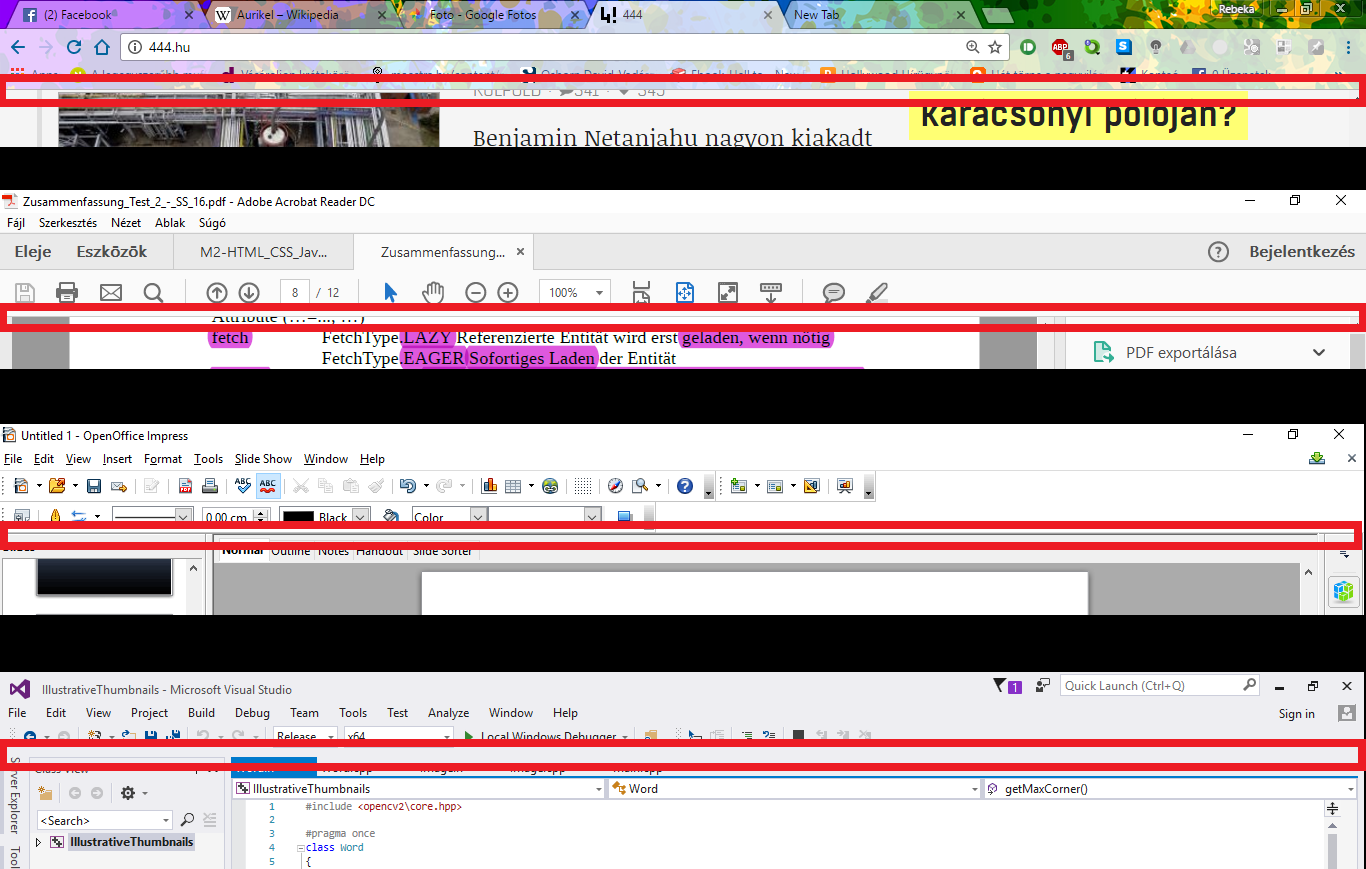
\includegraphics[width=\textwidth]{UIlines}
		\caption{Unicolor line at the edge of the UI area}
		\label{fig:lines}
	\end{figure}
	In case of predefined UI areas the method above works well, on the other hand, there are several specific occasions where it is not able to provide any results.
	Outstandingly, game applications usually use their own graphical UI, but even at more traditional applications it is plausible that the UI area is so overloaded or designed that no background line can be found.
	For this reason it is important to perform an additional checking loop, too.
	This step is based on the correlation value of the border and center's color histogram.
	The margin is split into thin slices.
	Initially the first slice near the border is examined.
	The histogram of this slice is then compared to the histogram of the center.
	If their correlation is high, it implies that the two areas are not significantly different, therefore nothing should be cut off, and so the algorithm returns.
	Alternatively, if low correlation is found, the examined strips are not part of the same unit, indicating that the slice is supposedly from within the UI area.
	In this case, the two histograms, the one with the first slice and the other from the center region, are kept for/as reference values.
	In the next step, the remaining slices are compared with the two reference histograms, starting at the border and heading towards the middle area.
	At the beginning the correlation with the border histogram is high and with the center is low, which shows that the slice is still in the UI area i.e. it matches the theme of the border widgets.
	This tendency reverses however as the slices approach the center regions.
	At the slice whose correlation with the center histogram is higher than the one with the border histogram, the algorithm stops, cuts all of the previously examined slices, and then terminates.
	Figure~\ref{fig:cropped} shows the borders between the content and UI regions found by the UI cropping heuristic.\par 
	\begin{figure}[h]
		\centering		
		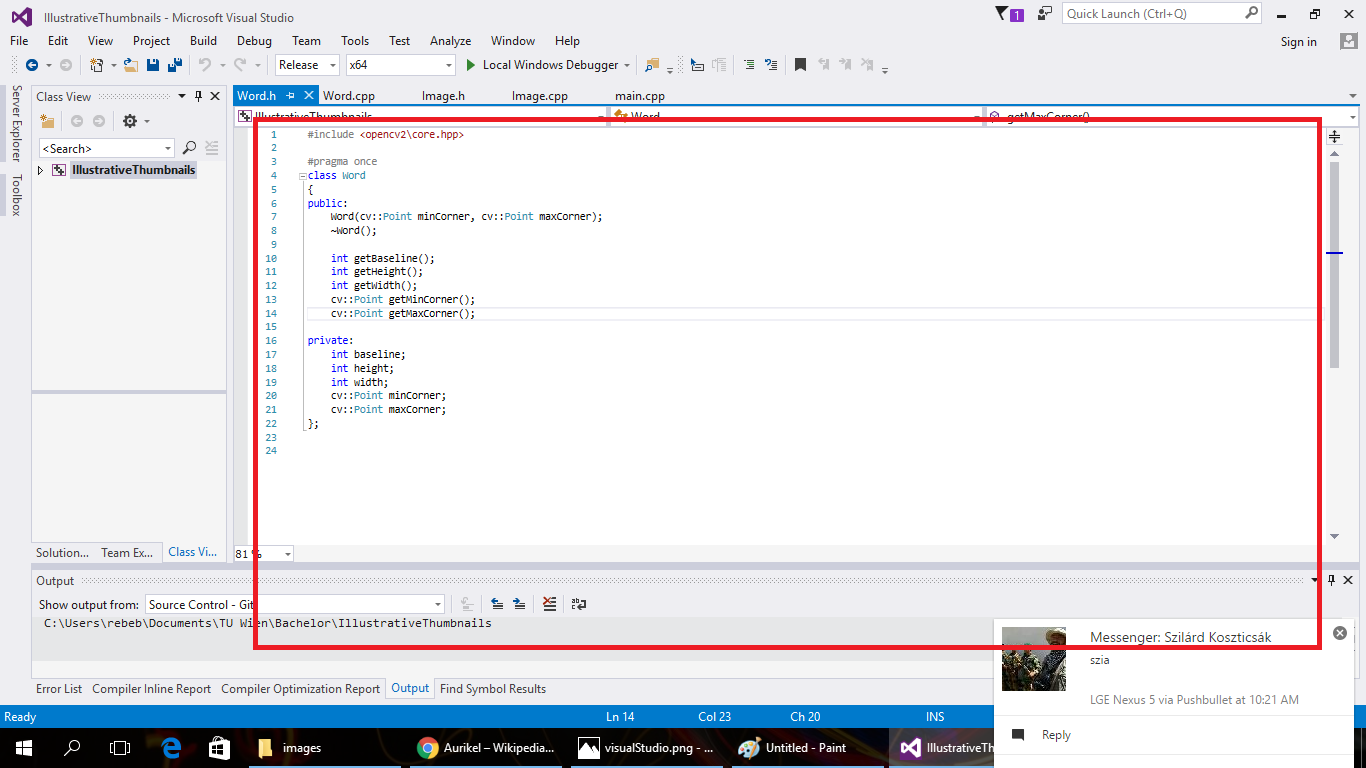
\includegraphics[width=0.5\textwidth]{cropped}
		\caption{The border of the content}
		\label{fig:cropped}
	\end{figure}
	%This method is executed four times.
	%In the first two cases the upper and the lower borders are %investigated.
	%The third and the fourth loop is adjusted to the sidebars.
	%In the first step not a horizontal but a vertical line is %searched, looking for a straight route, where the %background color of the sidebar takes the whole space %between the, already cropped, upper and lower borders of %the image.
	%Finally in the second checking loop the slices are defined %vertically and not horizontally this time. 
	
	\section{Saliency calculation}
	In order to ignore that parts of the source image that are actually unimportant, saliency calculation is applied.
	The saliency value of a pixel measures how important the pixel is, how noticeable it is and how much attention it affects for the human eye.
	A saliency map is a grayscale image where the high value of an area means that the region is more interesting than other pixels with lower values.
	There are, however, many definitions and approaches about which pixels should be evaluated as salient or not salient.
	In this case the saliency is calculated as presented by Niu et al.~\cite{niu2012image}. 
	There are two reasons, why this algorithm is chosen.
	First, it evaluates the low level visual informations.
	It means that only those pixels are valued as important that activate the low level human visual system, for example due to their sharp edges and color change characteristics.
	Secondly, it is scale invariant, so it is more robust than other similar but only singe scale approaches.\par 
	The algorithm converts the source into a uniform colorspace (Lu*v) first.
	After that, to make the approach scale invariant, a Gaussian contrast pyramid is built.
	It calculates the contrast value from the weighted sum of difference between the pixel and its neighborhood, using the L2 norm:	
	\[ C_{i,j,l}=\sum\limits_{q\in\Theta}w_{i,j,l}d(p_{i,j,l},p_{q}) \]
	\[ w_{i,j,l}=1-\left(\frac{r_{i,j,l}}{r_{l,max}}\right) \]
	where:
	\begin{center}
		\begin{conditions}
			C & Contrast value \\
			(i, j) & pixel coordinates \\
			l & pyramid level \\
			\Theta & neighborhood \\
			w & weight \\
			d & difference \\
			p & color of the pixel \\
			r & distance from the image center \\
			r_{l, max} & maximum possible distance on the image
		\end{conditions}
	\end{center}
	This approach needs to get slightly modified, in way that the calculation ignores the weighting value.
	The weighting parameter is used because of the fact that the central area of regular real word images is more important than the margin regions.
	When investigating computer screens, however, this is not the case.
	A screenshot often does not have a defined focus point where the most important information is shown.
	By using the weighting value, the focus would be on the inner window, despite the fact that there is no actual significant correlation between the importance of the data and its position on the screen.
	At the end, the importance value of each pixel is calculated by summing up all levels of the pyramid into one final saliency map.\par
	In the case of computer screens, texts are fairly common, and their information content is usually also very high.
	Therefore, it would be rather impractical not to reflect the importance of such text regions on the saliency map. 
	For that reason a further evaluation of the saliency map is needed, to check whether text areas were evaluated as important data.\par 
	The text recognition algorithm is based on the one introduced in ~\cite{chang2011associating}.
	For the first step the whole input image is horizontally blurred, so that the letters and the neighboring words form a string together.
	After that, all of these coherent strings are investigated and consorted depending on whether they are representations of actual words or if they derive from another visual feature of the source.
	The method that identifies the words examines two aspects.
	The first is if the strings are high enough but not too high to indicate real letters.
	Second, whether their width is not too small but also not too big to form at least one word but not an endless sentence.
	Both of these size examining values are parametrized, with their default value based on the size of one letter, as explained in the \hyperref[Implementation]{next chapter}. 
	The second loop evaluates the histograms of the area, where the strings were found.
	Normally the letters, if belonging to the same text data, have the same color, while the background, for optimal readability, does not change its color underneath the text, either.
	Therefore, the histograms of these areas are bimodal, namely one for the letters and one for the color of the background.
	To sum up, to identify a string as a word, it is not sufficient to pass the first check, it  also need  to have a corresponding special histogram to be labeled as word. 
	Figure~\ref{fig:strings} shows the output of the text detection algorithm. 
	The light blue color labels the possible word regions, the darker color denotes the actual words found by the algorithm.\par 
	\begin{figure}
		\centering
		\begin{subfigure}[b]{0.45\columnwidth}
			\centering
			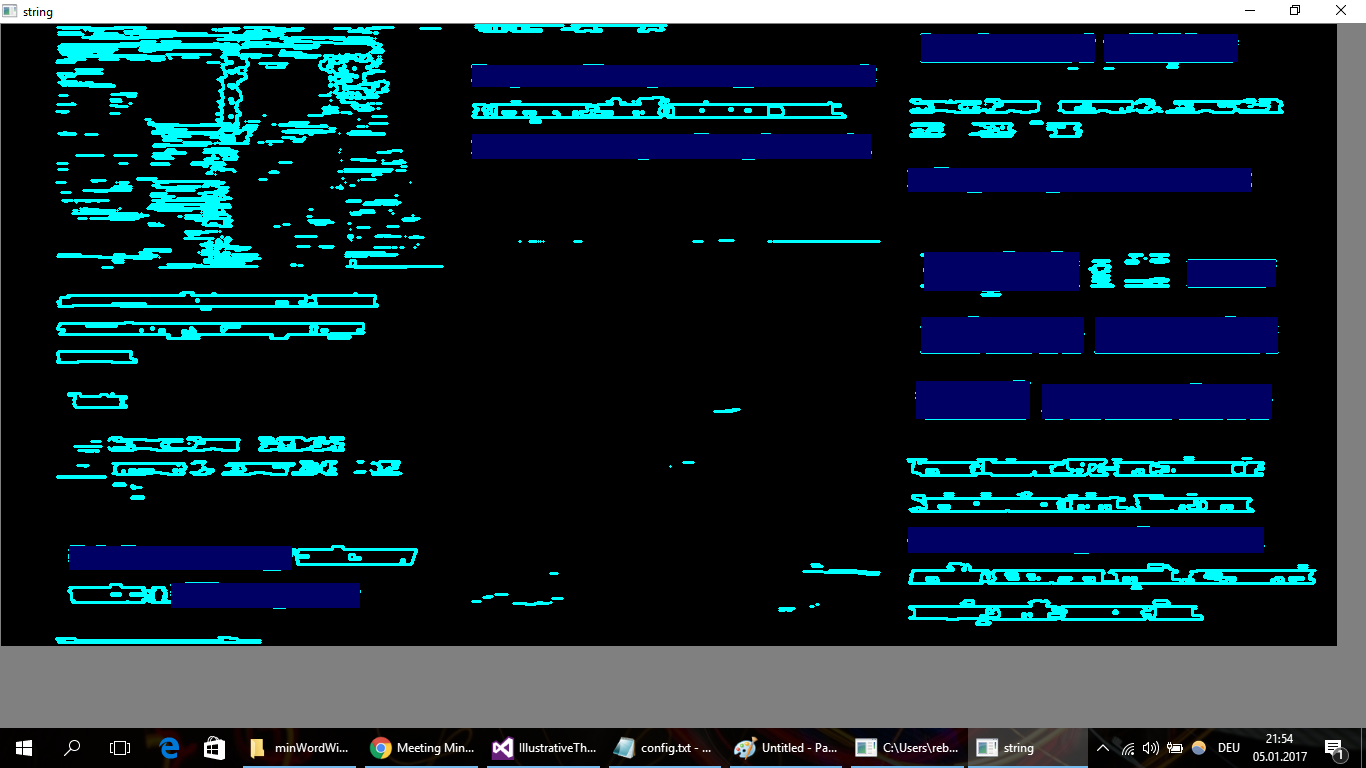
\includegraphics[width=\textwidth]{444}
			\subcaption{Input image}
			\label{fig:strings:org}
		\end{subfigure}
		\begin{subfigure}[b]{0.45\columnwidth}
			\centering
			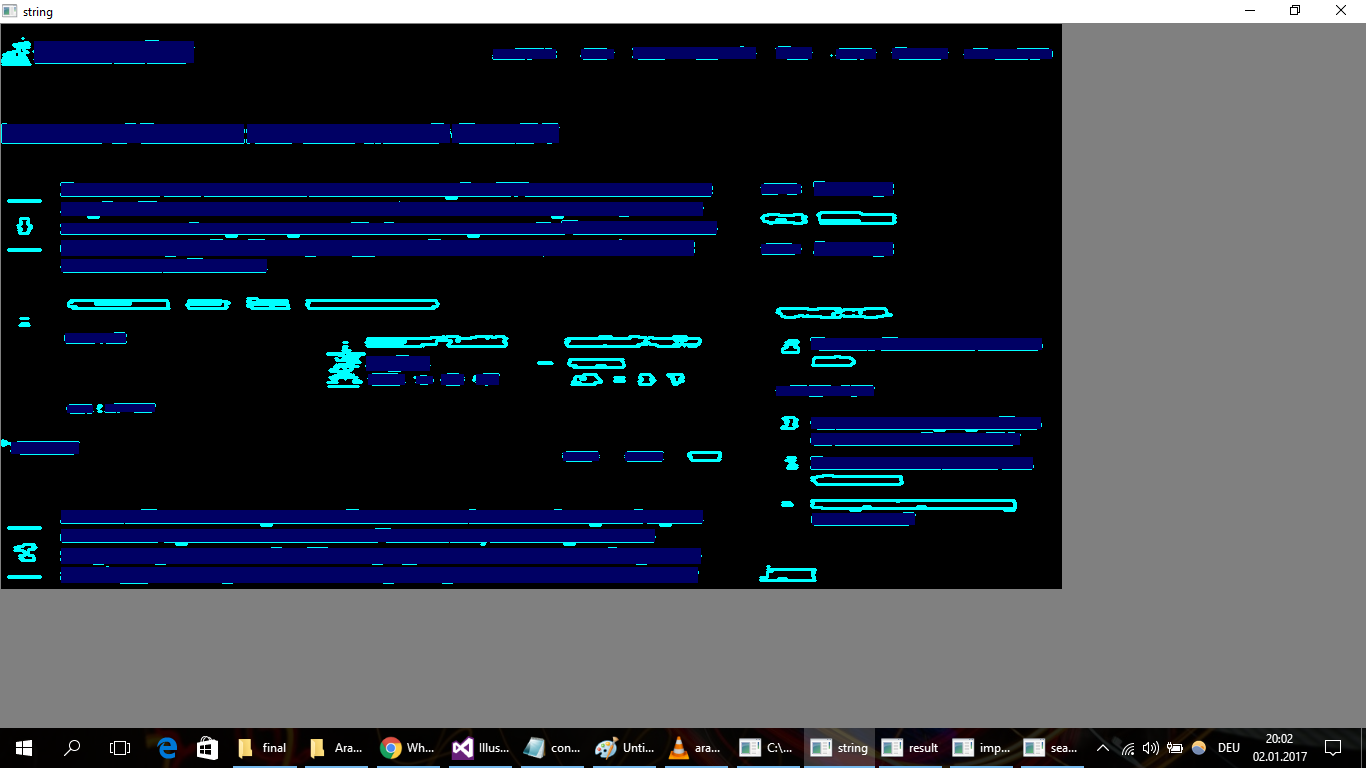
\includegraphics[width=\textwidth]{strings}
			\subcaption{Output}
		\end{subfigure}
		\caption{Result of the text detection algorithm applied on the given source}
		\label{fig:strings} % \label has to be placed AFTER \caption (or \subcaption) to produce correct cross-references.
	\end{figure}
	The last step for the calculation of the final saliency map, which is consequently used in the whole application, is to get the identified text regions weighted. 
	All area which passed the word checking test is automatically evaluated as highly important, and gets the highest saliency value.
	In addition, to make sure that even the space between the words remains undamaged, which is important because of greater readability, the area neighboring the text data is also weighted.
	Figure\ref{fig:saliency} is the final saliency map of Figure~\ref{fig:strings:org}.
	\begin{figure}[h]
		\centering		
		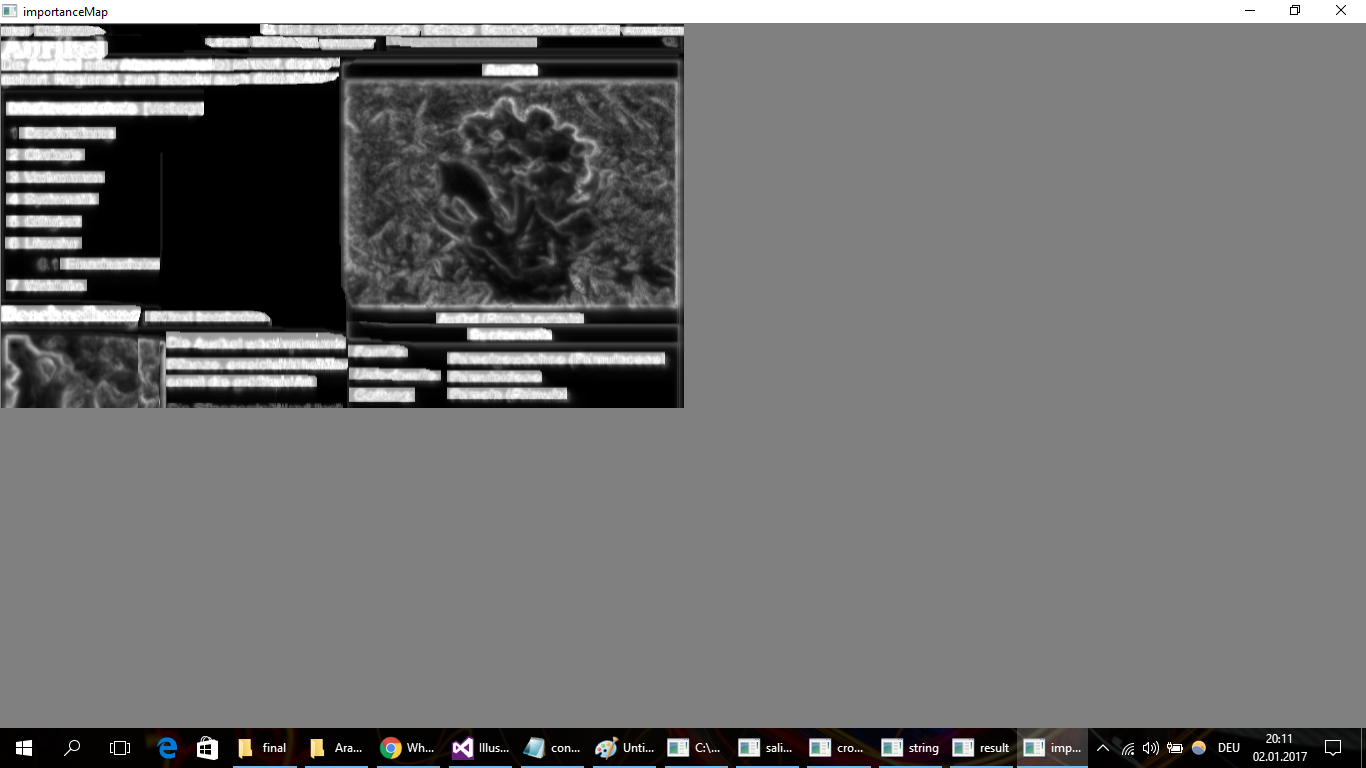
\includegraphics[width=0.5\textwidth]{saliency}
		\caption{The final saliency map}
		\label{fig:saliency}
	\end{figure}
	
	\section{Seam Carving}
	To resize the image without damaging the important regions, seam carving Forras is used.
	Seam carving calculates paths according to the saliency map, and eliminates those with minimal importance value.
	This step is repeated until the desired size is reached or the importance value of the chosen path exceeds a predefined threshold.
	Because seam carving does not necessary eliminates only the straight lines, the algorithm noticeably effects the layout of the unimportant regions.
	! Furthermore, if the whole image has very high salient values, the resulting seams do not have a remarkably smaller salient value than any straight line would have had when chosen randomly for resampling.
	To save the image from unnecessary artifacts and increase the application performance, a threshold value is defined as proposed in Forras.
	To reach the final output size common resampling is applied.\par 
	To find the most appropriate path, every possible solution need to be examined using the backpacking method.
	A path map is thus generated, where all past possibilities are stored, and that every new try can use as a look up.
	This way performance can be saved and the algorithm becomes faster.\par 
	! To find the next pixel of the path, five-neighborhood of the previous member is/are? examined. Five pieces of neighborh = are, a five-neighborhood + NOUN e.g. circle = is
	The algorithm runs from the top to the bottom, where the next member is chosen from the five nearest pixels of the next line.
	To calculate the costs of a possible switch between the columns the importance value of the neighboring pixels are weighted accordingly.
	In each case the chosen pixel is the one whose importance value with the weighting parameter is the smallest.
	Two paths per loop are calculated, one horizontally and one vertically, however, in the end only the pixels of the least salient path become eliminated.\par 
	Because the horizontal and vertical paths are eliminated independently, the picture being processed usually does not hold the aspect ratio.
	For this reason it is plausible that the weight and height parameters do not reach the output size or the threshold value at the same time.
	In this case the seam carving algorithm continues only for the remaining parameter until it reaches one of the conditions above. 
    The value of the threshold parameter is essential,	since it determines when the algorithm should /is to ha nem akarsz shouldot/ switch between seam carving and resampling. 
	It is calculated from the maximum salient path found after the first loop of the seam carving algorithm.
	Since with every loop one unsalient pixel is eliminated from the horizontal or from the vertical path, the relative saliency of the seams constantly increases.
	Therefore, in most cases, even the least salient seam will get more salient than the most salient seam of the original image. 
	The common resampling method eliminates the straight lines chosen from the source image until the desired size is reached.
	Seam carving is also applied to prevent paths with high salient value to be cut off.
	On the other hand, if the seams have as high importance value as any other of the source image, regular resampling has additional advantages.
	First, the algorithm is faster than the implemented seam carving method, and second, it applies an interpolating algorithm between the borders of the eliminated area, so in this case it ultimately saves more information than seam carving.   
	
	\chapter{Implementation}
	\label{implementation}
	The illustrative thumbnail creator application is developed in the programming language C++.
	Except the source image file browsing window, no operating system specific calls are performed.
	To make the application platform independent in the future, only this part needs customization.
	For image processing purposes Open Source Computer Vision Library (OpenCV) is used Forras.\par 
	!! OpenCV is apart from the computer vision also a machine learning library.     
	It has more than 2500 algorithms that can be used for image processing or for machine learning tasks, among object identification, finding similar images, image stitching and so on.
	Since the library offers support not exclusively for Windows, but also for Linux, Mac OS and Android, all methods taken from OpenCV can be regarded as platform independent functions.
	The library is applied when loading and saving the images, and to perform several image processing tasks like converting between color spaces, and image editing task such as blurring or filtering.
	The actual use of the library will be discussed in the section below.
	
	\section{Working Pipeline}
	In the following the actual implementation of the application is described.
	Apart from the functionalities mentioned in the previous chapter, other vital helper! Help methods are also discussed.
	To make the application configurable some essential parameters are set outside the application code. 
	A list of these parameters are highlighted below.
	
	\subsection{Image loading}
	Preceding the start of the thumbnail algorithm it is essential to load the source image.
	To make the application more flexible a Windows call is performed, allowing a new source image to be chosen after each start of the application.
	The type \texttt{OPENFILENAME} Forras, part of the Windows API, launches a file window to browse the required file.
	It shows only image files with the extension \texttt{.jpeg} or \texttt{.png}.
	After choosing the preferred source, the file path is established !"can be read"! and the OpenCV function \texttt{loadImage} opens the picture.
	
	\subsection{UI elimination}
	Near the margins the occurrence of UI elements is investigated.
	The application works with a configurable parameter, which defines the sections of the screen that are to be regarded as a margin area, using the default value of 20\%. 
	! Starting from the border towards the direction of the middle of the source, every row and thenafter, every column, are searched for a specific source line that first, has the same! same as what? color and second, a completely filled space between the vertical - later the horizontal - borders.
	Once accomplished, the OpenCV methods \texttt{rowRange} and \texttt{colRange} cut the input image.
	! After cutting, the histogram of the remaining margin area is examined and compared to the central region, !! where? the margin is split into thin slices.
	The function \texttt{calcHist} calculates histograms of the marginal and of the central window.
	If according to the function \texttt{compareHist}, which measures the correlation of two histograms,%\TODO{formel}
	they do not correlate, the comparison is performed on other slices that are consequently labeled as margin or central windows.
	If a slice is found that correlates with the margin histogram, the image is !cropped by! the slice again. 
	The parameters of correlation and the width of the slices are also configurable.
	According to testings, the best results are provided when the correlation is between 1.3 and 2 and the width is the 0.25\% of the window.
	
	\subsection{Saliancy map calculation}
	The saliency map is calculated from a Gaussian pyramid.
	But before building the pyramid the cropped source image has to get converted into a uniform colorspace.
	For this purpose the OpenCV function \texttt{cvtColor} is called.
	Then the levels of the pyramid are determined using the \texttt{pyrDown} method.
	Afterwards a contrast map is calculated with the L2 norm from the four neighboring pixels for each level.
	The last step is to merge the contrast images into one complete saliency map.
	Upscaling of the levels is performed, so they have the same size to the cropped image.
	The pixel value of the saliency map is given from the sum of pixels with the same coordinates for every level of the contrast pyramid. 
	In order to avoid any overflow, the pixel values are divided by the amount of pyramid levels.
	
	\subsection{Text detection}
	To find as many words as possible, the grayscale cropped source image is processed with the Laplacian operator, with the kernel size of three.
	As a result of the edge detection the layout of the letters are now highlighted.
	To make the series of letters related to each other, a horizontal blur is applied.
	The function \texttt{blur} is called. Although its kernel size is configurable, by default the height is set to one, the width to 15 pixels.
	Finally, the OpenCV function  \texttt{findContours} identifies the related regions and save their silhouette points into a 2 dimensional \texttt{vector}.
	For each region the width and height values are calculated.
	If a region is at least double as wide as high, the function proceeds with the examination of these attributes, namely whether they reach the minimum size for being an actual word.
	The size of the minimal word is configurable and by default set to 5x5, approximately the font size of 5pt, in order to be able to take even the smallest fonts into account.
	In case a region passes the test, it is marked as a possible word and is forwarded for further investigation.
	After labeling every region as word or non word region, the average height of the possible words is calculated.
	If the height of a possible word is significantly smaller or greater than the average, it is automatically sorted out.
	This confidence interval is also configurable and it is set to 50\% and 1000\%. 
	The maximal word height is defined generously in order to be able to find also the potentially large-sized titles and headlines.
	After the height test, the histogram of the possible word regions is examined.
	If it has exactly two accumulations, one for the color of the letters and one for the background, the region stays in the group of possible words, otherwise it is sorted out.
	Finally, the space above and below the possible words is investigated.
	Words are usually written in lines, with some space for readability placed between them. 
	Therefore if two possible word regions overlap i.e. have  common points at the top or at the bottom, it is inconceivable that the region in question represents a real words and thus is sorted out of the word list.
	When the final list is ready, the regions of the words are to be marked on the saliency map.
	The value of every text data pixel is automatically increased.
	At the very end the whole map is normalized with the OpenCV function \texttt{normalize} to avoid value overflow and other irregularities.  
	
	\subsection{Seam carving}
	Seam carving is implemented only in one, vertical, direction. 
	To be able to eliminate not only vertical but also horizontal seams, the cropped source image and the saliency map is rotated with the functions \texttt{transpose} and \texttt{flip}.
	For every loop a vertical and a horizontal seam is calculated, and the one with smaller saliency value is cut from the cropped source and from its saliency map.
	Until both sides reach the resampling value or the desired output size the seam carving algorithm is executed.
	The resampling value is calculated from the average pixel saliency value of the most salient seam on the cropped source image.
	The desired size and the resampling parameter are both customizable, they are set by default to 50\%. 
	The seam calculation algorithm works by writing a path map, where the previous paths and their saliency value are saved.
	At the beginning, the first row of the map is filled with the saliency values of the saliency map.
	Afterwards, for the next row the least salient successor of every pixel is searched, and the saliency value at the coordinates of the current pixel is added to the successor saliency value.
	If the new saliency value is smaller than the one already stored at the coordinates of the successor pixel, then the entry is updated and thus a better path is saved.
	By looking for the sucessor pixel the algorithm works with 5-neighborhood. 
	The saliency values of the five nearest pixels are weighted according to their position with $\sqrt{5}$, $\sqrt{2}$ and one.
	The pixel that is finally the least salient is chosen as successor.
	! When the algorithm finishes, in the end row of the path map the saliency values of the possible ways for starting at the first row are stored.
	! The final task is to find the smallest saliency value, and to follow the predecessor!? preceding/previous entities starting at the least salient pixel until the first row is reached again.
	The seam identified this way is afterwards eliminated not only from the cropped source image, but also from its saliency map.
	But if the saliency value of even the least expensive seam exceeds the resampling value, instead of cutting the path off, the usual resampling algorithm is applied using \texttt{resize} and the algorithm terminates.  
	
	\chapter{Results and Evaluation}
	To make the project configurable the application uses a \texttt{config.txt} file, where every parameter can be set as needed.
	In order to find the configuration, which provides reasonable results in as many cases as possible, several tests were performed.
	There is a test database including 14 pictures, showing seven different applications, captured on Windows 10.
	In the following the test cases of the elimination of UI elements, text detection and for the value of resampling threshold are presented and evaluated in respect to which of them is best able to provide the desired results.
	Then the application is compared to Adobe Photoshop Forras, with their advantages and disadvantages are described.
	At last the performace issues of the application is discussed briefly.
	\section{Elimination of UI elements} 
	Depending on the investigation area for UI elements, various regions of the border area may be cropped. 
	If the border region is defined too small (10\% of the image size) the algorithm terminates too early and not all UI widgets are cut off.
	But setting the border value too big (40\% of the image size) is also dangerous, because eventually the reference value for the central area can be chosen wrong, resulting in cropping from additional, non-border areas.
	Foto google, pdf \par 
	Starting from the histograms of the border area, the central area and the slices between them are sequentially compared, the value of their correlation is crucial for assigning them to one or another part of the image.
	If the correlation between the central area and the slice is set for too high, it means their correlation value has to be small (1), some content elements near the border can be eliminated, at low correlation however some UI widgets can be labeled as important content. 
	foto ppt, blizzard\par 
	The thickness of the slices influences how refined! alapos? throughout the algorithm is when searching through the border area.
	If the slices are really slim (5\% of the image size) the performance slightly decreases, but in exchange it is able to find a really close cropping point, i.e. where the UI and the content actually meets.
	foto desktop\par
	\section{Text detection}
	If the lines are already blurred on the grayscale image, the color of the letters and their area is slightly modified. 
	With the implementation of a threshold range a minimal pixel color value is defined that is in place to have the pixel labeled as possible text.
	If this parameter is small (50) any bright area can be classified as text, even if the given region is only neighboring a word.
	But if it is set to a high value (200), only the core of a word will reach it, so no region will actually contour its related word's shape.
	foto 444\par
	The properties of a possible word is also parametrized.
	The set of possible words needs to be sorted first, depending on how likely they are potential words when considering their size.
	The parameters for minimum height and width need to be chosen carefully, since if they are too big (width is set to 100, font size of 12pt, more than 6 letters or height to 20, font size of 14pt), almost every word will get excluded from the list.
	foto mindegy 
	From the set of the possible words the average word size is calculated, but thenafter it is still further customizable how much the words are allowed to vary from this value.
	For example if the allowed difference is set to 80\% the smaller words can easily get sorted out, while at 50\% they also manage to stay in the possible words set.
	foto pdf2\par 
	! With the inversion! visszaforditas of the algorithm, setting the weight of the words for negative, the functionality! hasznalhatosaga of the application can be changed.
	For experimental investigation the text areas were set non-salient, so only images and no words are saved. 
	When really small thumbnails are required, it  is advisable to save and present the image data instead of texts, since they would be illegible due to their minuscule size.  
	The experimental results are presented below.
	foto 
	\section{Resampling threshold}
	The resampling threshold determines when the application switches from seam carving to usual resampling. 
	If the value is small (0.1) only a few seam carving loops are performed, and the application behaves similar to a common down sampling algorithm.
	The performance is positively affected by fewer seam carving loops, but it also loses its advantage against simple resampling methods, with the important areas being no longer easily recognizable.
	When the threshold is set, however, to a bigger value, the application switches at the very end of the process.
	In this case the application works noticeably slower and additionally in causes more artifacts than usual resampling.
	foto diablo 
	\section{Comparison to Adobe Photoshop} 
	To compare the algorithm to an already existing tool the seam carving feature of Adobe Photoshop CS 5 Forras was used.
	There are two test scenarios; the first takes the same source to the illustrative thumbnail creator algorithm.
	The input image in the second case is however the cropped source image produced by this application after the elimination of the UI elements.
	In the first test it is investigated how seam carving invented for usual photos works on screenshots.
	Comparing  /photoshop/ images to outputs of the thumbnail algorithm, it is striking how much smaller and less readable the words appear.
	Because this project applies not only seam carving but also heuristics to cut off the border region, to compare the actual seam carving algorithms, Photoshop, to begin with seam calculation, it needs the same input as this application has.
	The second test scenario is in place for this reason.
	! The quality of the  output definitely improves, since an already smaller image needs to shrunk to the same size. / Hogyan  tud valami "same sized"-jára kicsinyedni?
	The main difference between the two methods seems to lay on the weighting of the content.
	This approach pays more attention to the text, with image data being easily ignored.
	Photoshop, however, attempts to sustain both regions, perhaps with a slightly more emphasize on the image content.
	Since the thumbnail creator algorithm has a ranking between the elements, holding texts before images, the output is not dubious: even in case of image data loss, the text remains readable.
	The output of Photoshop is rather disorganized, the text and image regions flow into each other.
	The images are significantly better recognizable, but in exchange the words are noticeably more damaged.  
	
	\section{Performance evaluation}
	The tests were performed on Windows 10 with CPU Intel i3-2310, 2.1GHZ and 2 Cores, using Grafic card AMD Radeon HD 7400M.
	During the tests some performance issues occurred, the application occasionally needed up to 3.5 minutes performance time, however remaining in a one-minute termination average.\par 
	The performance bottleneck is caused by seam calculation.
	Every time when a seam is eliminated, the whole saliency map is recalculated.
	Having a new saliency map the possible seam paths also need to get redetermined.
	If the UI cropping algorithm is not able to cut a bigger area or the resampling threshold is reached later, several seam carving loops are performed. 
	Therefore, screenshots with bigger and clearly defined UI areas have shorter run time, whereas inputs like images of gallery applications and of computer games take longer. 
	
	\chapter{Future Work}
	\label{futureWork}
	This application, according to the chapter above, is effective at creating illustrative thumbnails, but there are certain implementations to extend its scope. 
	There are two main improvement areas to investigate: performance and software methodology.
	Although the current application provides reasonable results, as described in the preceding chapters, there are several approaches, to make the present method even more robust and easier to use.
	The most important directions for development will be discussed in the following section.
	
	\section{Performance improvement} 
	The core task of a seam carving algorithm is the evaluation of the saliency map.
	Optimally, every pixel and every possible path are needed to be examined in order to find the most favorable path.
	Depending on the size of the input, visiting and checking all pixels individually can take a long time.
	This process can be get, however, easily parallelized.
	In 2007, Nvidia released a parallel computing platform, called CUDA Forras, which exploits the computing performance of the GPU.
	In addition, the CUDA system can be simply integrated into the current application, since it is developed for programming languages C, C++ and Fortran, that includes the C++ used in this project.   
	
	\section{Methodology improvement}
	An essential challenge in seam carving is the construction of the saliency map and the calculation of the seams. 
	The methods inplemented in the current project are able to handle most standard cases, on the other hand, with some improvements it has the potential to became more robust and usable in even more special cases.\par 
	There are several approaches that besides the low level pixel data examination, aims to find also semantical objects in the input.
	They are building on the observation, that some objects, for example faces, even if their coloring is not special, are very important for human viewers.
	The perceptual seam carving algorithm from Forras, based on the Human Attention Model, calculates not only the color changes but also the occurrence of facial information.
	It includes an already implemented feature of OpenCV, with which the application is able to generate a face map.
	The energy function, which calculates the pixel values in the saliency map, is then weighted with the data from the face map, so an even more detailed saliency map is constructed.\par 
	Furthermore, apart from the face information, Forras also uses gradient magnitude, Canny edge detection and Hugh line detection to make the saliency map as meaningful as possible. 
	It thoroughly examines both the semantic and the low level pixel data.
	There is, however, another method to evaluate the pixel information in an even more profound manner.
	! Putting the information into a context makes the measurements more accurate, because it controls for information extremities.! itt ezt akartad mondani?
	Consequently, no pixel will appear more important - or unimportant - than it really is.
	Forras obtains this with the calculation of a so-called neighborhood inhomogeneity factor, which denotes the amount of inhomogeneous neighbors of every pixel. 
	This approach helps to find the important areas inside an object, where a simple line detection algorithm fails i.e. indicate no salient regions.
	To find the coherent areas that later can be defined as objects, the use of a mean shift algorithm, as in Forras, would be effective. 
	Furthermore, it! what? makes the saliency calculation scale invariant!? constant/stable/unchanged?, and decreases the chance of finding misleadingly high important edges!.\par 
	When the saliency map is final, the next step is to calculate the seams.
	In this project seams are defined as paths with the width information of each pixel.
	On the other hand,  mitigation/moderation/ignoring-of of this rule can provide better results with less artifacts and also increases of performance, as obtained by Forras.
	This approach tries to find streams, seams wider than only one pixel, to eliminate bigger areas of the picture at once.
	Even if the cheapest seams are not neighboring, for the cost of eliminating a slightly greater salient region, the number of needed loops per image can be decreased.
	The most important precondition is that the stream is not allowed to cross any salient line or region, for example faces, so the relative saliency value still needs to stay low. \par
	In order to eliminate the possible artifacts caused by cutting of seams and streams an algorithm presented in Forras offers help.
	This approach is also based on saliency calculation.
	If there is a big area, which needs to be filled up, it investigates the saliency map and the texture of the neighboring regions.
	The most salient points are then labeled as anchor points; the actual task is to find !a way!? between these anchors and to color the background.
	In case of seam carving the goal is not to recreate the eliminated areas but with the above algorithm it is possible to make transition areas smoother.
	! If a stream is taken, a narrow, only a few pixel wide path can be !left behind!, to let the algorithm work.
	In the case of seams however the neighboring edges can be modified according to the filling method, taking some wider area around the seam as reference.\par 
	A further possibility to make the current algorithm faster and able to deal with the artifacts better is presented in Forras.
	This method has to slightly modify the pipeline of the project, since it employs usual resampling in the seam carving phase already.
	It classifies every pixel on the input image as foreground, very salient, related objects, and background, less salient, !probably split up parts of the image.!
	The seam carving method is applied only on the foreground data, the non-salient regions are processed with simple resampling. 
	With this approach the properties of the background have no influence on the actual sequence of seam.
	The calculation needs to take only the saliency values of the important foreground objects into account, therefore the resulting path will be more accurate and consist the most important regions of the picture.
	Furthermore, in this case a seam is shorter than it would be when it was be applied to the whole input, as it is only calculated for certain foreground objects, causing significantly smaller and less noticeable artifacts.
	As an additional favorable side effect, also the performance increases due to the decreased amount of areas to be considered for the seam calculation.    
	
	\chapter{Conclusion}
	To make thumbnails more illustrative and applicable even on small screens, a thumbnail creating method using seam carving was presented in this paper.
	In order to obtain the most informative results possible the saliency calculation was adjusted to the special requirements of a screenshot.
	In addition to seam calculation, the presence of UI elements on a computer screen were also taken into account.
	As a combined results of the customized seam carving algorithm and its extensions with other helpful methods such as UI part elimination, text recognition and common resampling, the created thumbnails are more illustrative than their usual relatives, since their information content is better recognizable and the text regions are easier to read. 
	
	% Remove following line for the final thesis.
	%% intro.tex
%% Copyright (C) 2014-2016 by Thomas Auzinger <thomas@auzinger.name>
%
% This work may be distributed and/or modified under the
% conditions of the LaTeX Project Public License, either version 1.3
% of this license or (at your option) any later version.
% The latest version of this license is in
%   http://www.latex-project.org/lppl.txt
% and version 1.3 or later is part of all distributions of LaTeX
% version 2005/12/01 or later.
%
% This work has the LPPL maintenance status `maintained'.
%
% The Current Maintainer of this work is Thomas Auzinger.
%
% This work consists of the files vutinfth.dtx and vutinfth.ins
% and the derived file vutinfth.cls.
% This work also consists of the file intro.tex.


\newacronym{ctan}{CTAN}{Comprehensive TeX Archive Network}
\newacronym{faq}{FAQ}{Frequently Asked Questions}
\newacronym{pdf}{PDF}{Portable Document Format}
\newacronym{svn}{SVN}{Subversion}
\newacronym{wysiwyg}{WYSIWYG}{What You See Is What You Get}

\newglossaryentry{texteditor}
{
  name={editor},
  description={A text editor is a type of program used for editing plain text files.}
}

\chapter{Introduction to \LaTeX}

Since \LaTeX\ is widely used in academia and industry, there exists a plethora of freely accessible introductions to the language.
Reading through the guide at \url{https://en.wikibooks.org/wiki/LaTeX} serves as a comprehensive overview for most of the functionality and is highly recommended before starting with a thesis in \LaTeX.

\section{Installation}

A full \LaTeX\ distribution\index{distribution} consists of not only of the binaries that convert the source files to the typeset documents, but also of a wide range of packages and their documentation.
Depending on the operating system, different implementations are available as shown in Table~\ref{tab:distrib}.
\textbf{Due to the large amount of packages that are in everyday use and due to their high interdependence, it is paramount to keep the installed distribution\index{distribution} up to date.}
Otherwise, obscure errors and tedious debugging ensue.

\begin{table}
  \centering
  \begin{tabular}{cccc}
    \toprule
    Distribution & Unix         & Windows      & MacOS        \\
    \midrule
    TeX Live     & \textbf{yes} & yes          & (yes)        \\
    MacTeX       & no           & no           & \textbf{yes} \\
    MikTeX       & no           & \textbf{yes} & no           \\
    \bottomrule
  \end{tabular}
  \caption{\TeX/\LaTeX\ distributions for different operating systems. Recomended choice in \textbf{bold}.}
  \label{tab:distrib} % \label has to be placed AFTER \caption to produce correct cross-references.
\end{table}

\section{Editors}

A multitude of \TeX\ \glspl{texteditor} are available differing in their editing models, their supported operating systems and their feature sets.
A comprehensive overview of \glspl{texteditor} can be found at the Wikipedia page  \url{https://en.wikipedia.org/wiki/Comparison_of_TeX_editors}.
TeXstudio (\url{http://texstudio.sourceforge.net/}) is recommended.
Most editors support the scrolling the typeset preview document to a location in the source document by \verb|Ctrl| clicking the location in the source document.

\section{Compilation}

Modern editors usually provide the compilation programs to generate \gls{pdf} documents and for most \LaTeX\ source files, this is sufficient.
More advanced \LaTeX\ functionality, such as glossaries and bibliographies, needs additional compilation steps, however.
It is also possible that errors in the compilation process invalidate intermediate files and force subsequent compilation runs to fail.
It is advisable to delete intermediate files (\verb|.aux|, \verb|.bbl|, etc.), if errors occur and persist.
All files that are not generated by the user are automatically regenerated.
To compile the current document, the steps as shown in Table~\ref{tab:compile} have to be taken.


\begin{table}
  \centering
  \begin{tabular}{rl}
    \toprule
    & Description \\
    \midrule
    1 & Scan for refs, toc/lof/lot/loa items and cites \\
    2 & Build the bibliography     \\
    3 & Link refs and build the toc/lof/lot/loa \\
    4 & Link the bibliography \\
    5 & Build the glossary \\
    6 & Build the acronyms \\
    7 & Build the index \\
    8 & Link the glossary, acronyms, and the index \\
    9 & Link the bookmarks \\
    \midrule
    & Command \\
    \midrule
    1 & \verb|pdflatex.exe  example| \\
    2 & \verb|bibtex.exe    example| \\
    3 & \verb|pdflatex.exe  example| \\
    4 & \verb|pdflatex.exe  example| \\
    5 & \verb|makeindex.exe -t example.glg -s example.ist| \\
      & \verb|              -o example.gls example.glo| \\
    6 & \verb|makeindex.exe -t example.alg -s example.ist| \\
      & \verb|              -o example.acr example.acn| \\
    7 & \verb|makeindex.exe -t example.ilg -o example.ind example.idx| \\
    8 & \verb|pdflatex.exe  example| \\
    9 & \verb|pdflatex.exe  example| \\
    \bottomrule
  \end{tabular}
  \caption{Compilation steps for this document. The following abbreviations were used: table of contents (toc), list of figures (lof), list of tables (lot), list of algorithms (loa).}
  \label{tab:compile} % \label has to be placed AFTER \caption to produce correct cross-references.
\end{table}


\section{Basic Functionality}

In this section, various examples are given of the fundamental building blocks used in a thesis.
Many \LaTeX\ commands have a rich set of options that can be supplied as optional arguments.
The documentation of each command should be consulted to get an impression of the full spectrum of its functionality.

\subsection{Floats}

'Two main categories of page elements can be differentiated in the usual \LaTeX\ workflow: \textit{(i)} the main stream of text and \textit{(ii)} floating containers that are positioned at convenient positions throughout the document.
In most cases, tables, plots, and images are put into such containers since they are usually positioned at the top or bottom of pages.
These are realized jtk dgm,fsds by the two environments \verb|figure| and \verb|table|, which also provide functionality for cross-referencing (see Table~\ref{tab:intro} and Figure~\ref{fig:intro}) and the generation of corresponding entries in the list of figures and the list of tables.
Note that these environments solely act as containers and can be assigned arbitrary content.

\subsection{Tables}

A table in \LaTeX\ is created by using a \verb|tabular| environment or any of its extensions, e.g., \verb|tabularx|.
The commands \verb|\multirow| and \verb|\multicolumn| allow table elements to span multiple rows and columns.

\begin{table}[h] % placement specifier
  \centering
  \begin{tabular}{lll}
    \toprule
    \multicolumn{2}{c}{Position} \\
    \cmidrule{1-2} % partial horizontal rule
    Group & Abbrev & Name \\
    \midrule
    Goalkeeper & GK & Paul Robinson \\
    \midrule
    \multirow{4}{*}{Defenders} & LB & Lucus Radebe \\
                               & DC & Michael Duburry \\
                               & DC & Dominic Matteo \\
                               & RB & Didier Domi \\
    \midrule
    \multirow{3}{*}{Midfielders} & MC & David Batty \\
                                 & MC & Eirik Bakke \\
                                 & MC & Jody Morris \\
    \midrule
    Forward & FW & Jamie McMaster \\
    \midrule
    \multirow{2}{*}{Strikers} & ST & Alan Smith \\
                              & ST & Mark Viduka \\
    \bottomrule
  \end{tabular}
  \caption{Adapted example from the \LaTeX guide at \url{https://en.wikibooks.org/wiki/LaTeX/Tables}. This example uses rules specific to the \texttt{booktabs} package and employs the multi-row functionality of the \texttt{multirow} package.}
  \label{tab:intro} % \label has to be placed AFTER \caption to produce correct cross-references.
\end{table}

\subsection{Images}

An image is added to a document via the \verb|\includegraphics| command as shown in Figure~\ref{fig:intro}.
The \verb|\subcaption| command can be used to reference subfigures, such as Figure~\ref{fig:intro:full width} and~\ref{fig:intro:half width}.

\begin{figure}[h]
  \centering
  \begin{subfigure}[b]{0.45\columnwidth}
    \centering
    
\includegraphics[width=\textwidth]{TU_INF_Logo_gray}
    \subcaption{The header logo at text width.}
    \label{fig:intro:full width}
  \end{subfigure}
  \begin{subfigure}[b]{0.45\columnwidth}
    \centering
    
\includegraphics[width=0.5\textwidth]{TU_INF_Logo_gray}
    \subcaption{The header logo at half the text width.}
    \label{fig:intro:half width}
  \end{subfigure}
  \caption{The header logo at different sizes.}
  \label{fig:intro} % \label has to be placed AFTER \caption (or \subcaption) to produce correct cross-references.
\end{figure}

\subsection{Mathematical Expressions}

One of the original motivation to create the \TeX\ system was the need for mathematical typesetting.
To this day, \LaTeX\ is the preferred system to write math-heavy documents and a wide variety of functions aids the author in this task.
A mathematical expression can be inserted inline as $\sum_{n=1}^{\infty} \frac{1}{n^2} = \frac{\pi^2}{6}$ outside of the text stream as \[ \sum_{n=1}^{\infty} \frac{1}{n^2} = \frac{\pi^2}{6} \] or as numbered equation with
\begin{equation}
\sum_{n=1}^{\infty} \frac{1}{n^2} = \frac{\pi^2}{6}.
\end{equation}

\subsection{Pseudo Code}

The presentation of algorithms can be achieved with various packages; the most popular are \verb|algorithmic|, \verb|algorithm2e|, \verb|algorithmicx|, or \verb|algpseudocode|.
An overview is given at \url{https://tex.stackexchange.com/questions/229355}.
An example of the use of the \verb|alogrithm2e| package is given with Algorithm~\ref{alg:gauss-seidel}.

\begin{algorithm}
  \SetKw{BreakFor}{break for}
  \KwIn{A scalar~$\epsilon$, a matrix $\mathbf{A} = (a_{ij})$, a vector $\vec{b}$, and an initial vector $\vec{x}^{(0)}$}
  \KwOut{$\vec{x}^{(n)}$ with $\mathbf{A} \vec{x}^{(n)} \approx \vec{b}$}
  \For{$k\leftarrow 1$ \KwTo maximum iterations}
  {
     \For{$i\leftarrow 1$ \KwTo $n$}
     {
        $x_i^{(k)} = \frac{1}{a_{ii}} \left(b_i-\sum_{j<i} a_{ij} x_j^{(k)} - \sum_{j>i} a_{ij} x_j^{(k-1)} \right)$\;
     }
     \If{$\lvert\vec{x}^{(k)}-\vec{x}^{(k-1)}\rvert < \epsilon$}
     {\BreakFor\;}
  }
  \Return{$\vec{x}^{(k)}$\;}
  \caption{Gauss-Seidel}
  \label{alg:gauss-seidel} % \label has to be placed AFTER \caption to produce correct cross-references.
\end{algorithm}

\section{Bibliography}

The referencing of prior work is a fundamental requirement of academic writing and well supported by \LaTeX.
The \textsc{Bib}\TeX\ reference management software is the most commonly used system for this purpose.
Using the \verb|\cite| command, it is possible to reference entries in a \verb|.bib| file out of the text stream, e.g., as~\cite{Turing1936}.
The generation of the formatted bibliography needs a separate execution of \verb|bibtex.exe| (see Table~\ref{tab:compile}).

\section{Table of Contents}

The table of contents is automatically built by successive runs of the compilation, e.g., of \verb|pdflatex.exe|.
The command \verb|\setsecnumdepth| allows the specification of the depth of the table of contents and additional entries can be added to the table of contents using \verb|\addcontentsline|.
The starred versions of the sectioning commands, i.e., \verb|\chapter*|, \verb|\section*|, etc., remove the corresponding entry from the table of contents.

\section{Acronyms / Glossary / Index}

The list of acronyms, the glossary, and the index need to be built with a separate execution of \verb|makeindex| (see Table~\ref{tab:compile}).
Acronyms have to be specified with \verb|\newacronym| while glossary entries use \verb|\newglossaryentry|.
Both are then used in the document content with one of the variants of \verb|\gls|, such as \verb|\Gls|, \verb|\glspl|, or \verb|\Glspl|.
Index items are simply generated by placing \verb|\index|\marg{entry} next to all the words that correspond to the index entry \meta{entry}.
Note that many enhancements exist for these functionalities and the documentation of the \verb|makeindex| and the \verb|glossaries| packages should be consulted.

\section{Tips}

Since \TeX\ and its successors do not employ a \gls{wysiwyg} editing scheme, several guidelines improve the readability of the source content:
\begin{itemize}
\item Each sentence in the source text should start with a new line.
      This helps not only the user navigation through the text, but also enables revision control systems (e.g. \gls{svn}, Git) to show the exact changes authored by different users.
      Paragraphs are separated by one (or more) empty lines.
\item Environments, which are defined by a matching pair of \verb|\begin{name}| and \verb|\end{name}|, can be indented by whitespace to show their hierarchical structure.
\item In most cases, the explicit use of whitespace (e.g. by adding \verb|\hspace{4em}| or \verb|\vspace{1.5cm}|) violates typographic guidelines and rules.
      Explicit formatting should only be employed as a last resort and, most likely, better ways to achieve the desired layout can be found by a quick web search.
\item The use of bold or italic text is generally not supported by typographic considerations and the semantically meaningful \verb|\emph{|\texttt{$\dots$}\verb|}| should be used.
\end{itemize}

The predominant application of the \LaTeX\ system is the generation of \gls{pdf} files via the \textsc{Pdf}\LaTeX\ binaries.
In the current version of \textsc{Pdf}\LaTeX, it is possible that absolute file paths and user account names are embedded in the final \gls{pdf} document.
While this poses only a minor security issue for all documents, it is highly problematic for double blind reviews.
The process shown in Table~\ref{tab:ps2pdf} can be employed to strip all private information from the final \gls{pdf} document.

\begin{table}[h]
  \centering
  \begin{tabular}{rl}
  \toprule
  & Command \\
  \midrule
  1 & Rename the \gls{pdf} document \verb|final.pdf| to \verb|final.ps|. \\
  2 & Execute the following command: \\
    & \verb|ps2pdf -dPDFSETTINGS#/prepress ^| \\
    & \verb| -dCompatibilityLevel#1.4 ^| \\
    & \verb| -dAutoFilterColorImages#false ^| \\
    & \verb| -dAutoFilterGrayImages#false ^| \\
    & \verb| -dColorImageFilter#/FlateEncode ^| \\
    & \verb| -dGrayImageFilter#/FlateEncode ^| \\
    & \verb| -dMonoImageFilter#/FlateEncode ^| \\
    & \verb| -dDownsampleColorImages#false ^| \\
    & \verb| -dDownsampleGrayImages#false ^| \\
    & \verb| final.ps final.pdf| \\
  \bottomrule
  \end{tabular}

  On Unix-based systems, replace \verb|#| with \verb|=| and \verb|^| with \verb|\|.
  \caption{Anonymization of \gls{pdf} documents.}
  \label{tab:ps2pdf}
\end{table}

\section{Resources}

\subsection{Useful Links}

In the following, a listing of useful web resources is given.
\begin{description}
\item[\url{https://en.wikibooks.org/wiki/LaTeX}] An extensive wiki-based guide to \LaTeX.
\item[\url{http://www.tex.ac.uk/faq}] A (huge) set of \gls{faq} about \TeX\ and \LaTeX.
\item[\url{https://tex.stackexchange.com/}] The definitive user forum for non-trivial \LaTeX-related questions and answers.
\end{description}

\subsection[Comprehensive TeX Archive Network]{\gls{ctan}}

The \gls{ctan} is the official repository for all \TeX\ related material.
It can be accessed via \url{https://www.ctan.org/} and hosts (among other things) a huge variety of packages that provide extended functionality for \TeX\ and its successors.
Note that most packages contain \gls{pdf} documentation that can be directly accessed via \gls{ctan}.

In the following, a short, non-exhaustive list of relevant \gls{ctan}-hosted packages is given together with their relative path.
\begin{description}[itemsep=0ex]
\item[\href{https://www.ctan.org/pkg/algorithm2e}{algorithm2e}] Functionality for writing pseudo code.
\item[\href{https://www.ctan.org/pkg/amsmath}{amsmath}] Enhanced functionality for typesetting mathematical expressions.
\item[\href{https://www.ctan.org/pkg/amsfonts}{amssymb}] Provides a multitude of mathematical symbols.
\item[\href{https://www.ctan.org/pkg/booktabs}{booktabs}] Improved typesetting of tables.
\item[\href{https://www.ctan.org/pkg/enumitem}{enumitem}] Control over the layout of lists (\verb|itemize|, \verb|enumerate|, \verb|description|).
\item[\href{https://www.ctan.org/pkg/fontenc}{fontenc}] Determines font encoding of the output.
\item[\href{https://www.ctan.org/pkg/glossaries}{glossaries}] Create glossaries and list of acronyms.
\item[\href{https://www.ctan.org/pkg/graphicx}{graphicx}] Insert images into the document.
\item[\href{https://www.ctan.org/pkg/inputenc}{inputenc}] Determines encoding of the input.
\item[\href{https://www.ctan.org/pkg/l2tabu}{l2tabu}] A description of bad practices when using \LaTeX.
\item[\href{https://www.ctan.org/pkg/mathtools}{mathtools}] Further extension of mathematical typesetting.
\item[\href{https://www.ctan.org/pkg/memoir}{memoir}] The document class on upon which the \verb|vutinfth| document class is based.
\item[\href{https://www.ctan.org/pkg/multirow}{multirow}] Allows table elements to span several rows.
\item[\href{https://www.ctan.org/pkg/pgfplots}{pgfplots}] Function plot drawings.
\item[\href{https://www.ctan.org/pkg/pgf}{pgf/TikZ}] Creating graphics inside \LaTeX\ documents.
\item[\href{https://www.ctan.org/pkg/subcaption}{subcaption}] Allows the use of subfigures and enables their referencing.
\item[\href{https://www.ctan.org/tex-archive/info/symbols/comprehensive/}{symbols/comprehensive}] A listing of around 5000 symbols that can be used with \LaTeX.
\item[\href{https://www.ctan.org/pkg/voss-mathmode}{voss-mathmode}] A comprehensive overview of typesetting mathematics in \LaTeX.
\item[\href{https://www.ctan.org/pkg/xcolor}{xcolor}] Allows the definition and use of colors.
\end{description} % A short introduction to LaTeX.
	
	\backmatter
	
	% Use an optional list of figures.
	\listoffigures % Starred version, i.e., \listoffigures*, removes the toc entry.
	
	% Use an optional list of tables.
	\cleardoublepage % Start list of tables on the next empty right hand page.
	\listoftables % Starred version, i.e., \listoftables*, removes the toc entry.
	
	% Use an optional list of alogrithms.
	\listofalgorithms
	\addcontentsline{toc}{chapter}{List of Algorithms}
	
	% Add an index.
	\printindex
	
	% Add a glossary.
	\printglossaries
	
	% Add a bibliography.
	\bibliographystyle{alpha}
	\bibliography{intro}
	
\end{document}